\documentclass[14pt]{extbook}
\usepackage{multicol, enumerate, enumitem, hyperref, color, soul, setspace, parskip, fancyhdr} %General Packages
\usepackage{amssymb, amsthm, amsmath, latexsym, units, mathtools} %Math Packages
\everymath{\displaystyle} %All math in Display Style
% Packages with additional options
\usepackage[headsep=0.5cm,headheight=12pt, left=1 in,right= 1 in,top= 1 in,bottom= 1 in]{geometry}
\usepackage[usenames,dvipsnames]{xcolor}
\usepackage{dashrule}  % Package to use the command below to create lines between items
\newcommand{\litem}[1]{\item#1\hspace*{-1cm}\rule{\textwidth}{0.4pt}}
\pagestyle{fancy}
\lhead{Progress Quiz 1}
\chead{}
\rhead{Version C}
\lfoot{4082-7053}
\cfoot{}
\rfoot{test}
\begin{document}

\begin{enumerate}
\litem{
Write the equation of the line in the graph below in Standard form $Ax+By=C$. Then, choose the intervals that contain $A, B, \text{ and } C$.
\begin{center}
    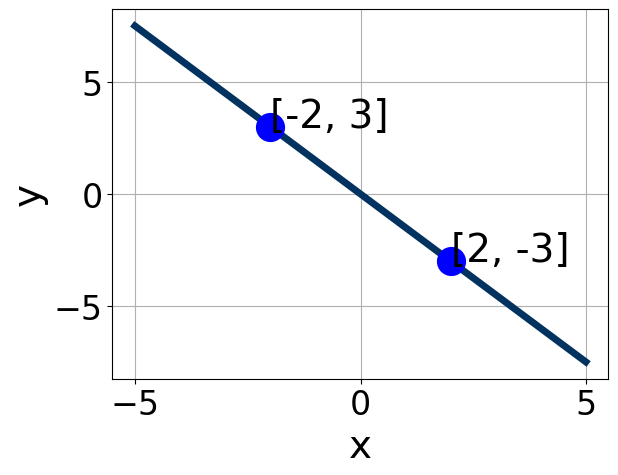
\includegraphics[width=0.5\textwidth]{../Figures/linearGraphToStandardC.png}
\end{center}
\begin{enumerate}[label=\Alph*.]
\item \( A \in [3, 11], \hspace{3mm} B \in [-4.9, -2.83], \text{ and } \hspace{3mm} C \in [-12, -3] \)
\item \( A \in [-3.25, 3.75], \hspace{3mm} B \in [-2.37, -0.05], \text{ and } \hspace{3mm} C \in [-2, 1] \)
\item \( A \in [-3.25, 3.75], \hspace{3mm} B \in [0.66, 1.09], \text{ and } \hspace{3mm} C \in [1, 5] \)
\item \( A \in [-8, -4], \hspace{3mm} B \in [3.45, 4.54], \text{ and } \hspace{3mm} C \in [3, 12] \)
\item \( A \in [3, 11], \hspace{3mm} B \in [3.45, 4.54], \text{ and } \hspace{3mm} C \in [3, 12] \)

\end{enumerate} }
\litem{
Find the equation of the line described below. Write the linear equation as $ y=mx+b $ and choose the intervals that contain $m$ and $b$.\[ \text{Parallel to } 6 x + 5 y = 8 \text{ and passing through the point } (-2, 4). \]\begin{enumerate}[label=\Alph*.]
\item \( m \in [-2.17, -1.14] \hspace*{3mm} b \in [1.07, 2.48] \)
\item \( m \in [0.37, 1.88] \hspace*{3mm} b \in [6.29, 6.78] \)
\item \( m \in [-2.17, -1.14] \hspace*{3mm} b \in [5.73, 6.3] \)
\item \( m \in [-2.17, -1.14] \hspace*{3mm} b \in [-1.78, -1.14] \)
\item \( m \in [-0.97, -0.67] \hspace*{3mm} b \in [1.07, 2.48] \)

\end{enumerate} }
\litem{
Solve the equation below. Then, choose the interval that contains the solution.\[ -18(15x + 16) = -6(-10x -9) \]\begin{enumerate}[label=\Alph*.]
\item \( x \in [-0.77, -0.68] \)
\item \( x \in [-1.13, -1.11] \)
\item \( x \in [0.66, 0.74] \)
\item \( x \in [-1.04, -1] \)
\item \( \text{There are no real solutions.} \)

\end{enumerate} }
\litem{
Find the equation of the line described below. Write the linear equation as $ y=mx+b $ and choose the intervals that contain $m$ and $b$.\[ \text{Perpendicular to } 3 x - 8 y = 6 \text{ and passing through the point } (-10, 8). \]\begin{enumerate}[label=\Alph*.]
\item \( m \in [-2.38, 2.62] \hspace*{3mm} b \in [-19.57, -18.5] \)
\item \( m \in [-2.67, -0.67] \hspace*{3mm} b \in [-19.57, -18.5] \)
\item \( m \in [1.67, 5.67] \hspace*{3mm} b \in [33.55, 34.88] \)
\item \( m \in [-2.67, -0.67] \hspace*{3mm} b \in [16.67, 18.61] \)
\item \( m \in [-2.67, -0.67] \hspace*{3mm} b \in [18.32, 18.75] \)

\end{enumerate} }
\litem{
Write the equation of the line in the graph below in Standard form $Ax+By=C$. Then, choose the intervals that contain $A, B, \text{ and } C$.
\begin{center}
    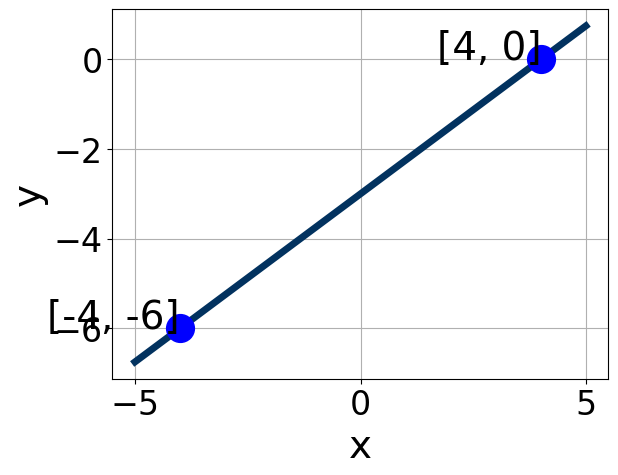
\includegraphics[width=0.5\textwidth]{../Figures/linearGraphToStandardCopyC.png}
\end{center}
\begin{enumerate}[label=\Alph*.]
\item \( A \in [-3.25, 0.75], \hspace{3mm} B \in [-1.6, -0.4], \text{ and } \hspace{3mm} C \in [-3, 4] \)
\item \( A \in [1, 10], \hspace{3mm} B \in [-7.5, -3.1], \text{ and } \hspace{3mm} C \in [-3, 4] \)
\item \( A \in [-3.25, 0.75], \hspace{3mm} B \in [0.6, 2.4], \text{ and } \hspace{3mm} C \in [-3, 4] \)
\item \( A \in [-11, -3], \hspace{3mm} B \in [3.3, 4.1], \text{ and } \hspace{3mm} C \in [-3, 4] \)
\item \( A \in [1, 10], \hspace{3mm} B \in [3.3, 4.1], \text{ and } \hspace{3mm} C \in [-3, 4] \)

\end{enumerate} }
\litem{
Solve the linear equation below. Then, choose the interval that contains the solution.\[ \frac{3x -6}{5} - \frac{-8x -7}{3} = \frac{6x -7}{4} \]\begin{enumerate}[label=\Alph*.]
\item \( x \in [-3.1, -0.6] \)
\item \( x \in [-0.3, 1.6] \)
\item \( x \in [-6.1, -3.5] \)
\item \( x \in [-1.3, -0.2] \)
\item \( \text{There are no real solutions.} \)

\end{enumerate} }
\litem{
Solve the equation below. Then, choose the interval that contains the solution.\[ -8(-5x -17) = -2(15x + 6) \]\begin{enumerate}[label=\Alph*.]
\item \( x \in [-12.68, -12.18] \)
\item \( x \in [1.43, 2.25] \)
\item \( x \in [-2.87, -1.96] \)
\item \( x \in [-2.03, -1.43] \)
\item \( \text{There are no real solutions.} \)

\end{enumerate} }
\litem{
First, find the equation of the line containing the two points below. Then, write the equation as $ y=mx+b $ and choose the intervals that contain $m$ and $b$.\[ (-10, -2) \text{ and } (-2, -3) \]\begin{enumerate}[label=\Alph*.]
\item \( m \in [0, 0.33] \hspace*{3mm} b \in [-3.21, -2] \)
\item \( m \in [-0.2, -0] \hspace*{3mm} b \in [-3.94, -2.88] \)
\item \( m \in [-0.2, -0] \hspace*{3mm} b \in [-1.21, -0.95] \)
\item \( m \in [-0.2, -0] \hspace*{3mm} b \in [3.1, 3.26] \)
\item \( m \in [-0.2, -0] \hspace*{3mm} b \in [7.72, 8.16] \)

\end{enumerate} }
\litem{
Solve the linear equation below. Then, choose the interval that contains the solution.\[ \frac{6x + 3}{8} - \frac{-4x + 7}{4} = \frac{4x + 4}{3} \]\begin{enumerate}[label=\Alph*.]
\item \( x \in [18.4, 19.8] \)
\item \( x \in [-2.6, -1.7] \)
\item \( x \in [6.3, 7.8] \)
\item \( x \in [0.1, 1.1] \)
\item \( \text{There are no real solutions.} \)

\end{enumerate} }
\litem{
First, find the equation of the line containing the two points below. Then, write the equation as $ y=mx+b $ and choose the intervals that contain $m$ and $b$.\[ (2, 9) \text{ and } (4, 8) \]\begin{enumerate}[label=\Alph*.]
\item \( m \in [-1.67, 0.11] \hspace*{3mm} b \in [6.93, 7.51] \)
\item \( m \in [-1.67, 0.11] \hspace*{3mm} b \in [3.45, 4.1] \)
\item \( m \in [-1.67, 0.11] \hspace*{3mm} b \in [-10.32, -9.12] \)
\item \( m \in [-1.67, 0.11] \hspace*{3mm} b \in [7.88, 12.14] \)
\item \( m \in [-0.12, 2.04] \hspace*{3mm} b \in [5.92, 6.58] \)

\end{enumerate} }
\end{enumerate}

\end{document}